\documentclass[12pt]{article}
\usepackage{uwyo_report} % loads in all the specific formatting
\usepackage{amsmath}
\usepackage{amssymb}
\usepackage{float}
\usepackage{multicol}


% if you want other packages, put them here

% macro for typesetting the word BibTeX
\def\BibTeX{{\rm B\kern-.05em{\sc i\kern-.025em b}\kern-.08em
   T\kern-.1667em\lower.7ex\hbox{E}\kern-.125emX}}


\begin{document}

\title{EE 5450  Project 01: Simultaneous Monocular Calibration and Pose Estimation}

\author{David R. Mohler}

%\date{December 7, 1941}

\maketitle

\section{Introduction} 
Determination of the pose of rigid objects within images is a common problem within many practical application of computer vision, robotics, computer graphics, etc. The following set of experiments are focused on the application of the simultaneous monocular calibration and pose estimation algorithm to a series of images of rigid objects with known dimensions and correspondence points. From this known data, the algorithm is capable of calibrating a single monocular camera with a fixed focal length. The calibration enables simultaneous discovery of the pose of the viewed object, and from this generate a three dimensional representation of that same object.  
%In this project we will demonstrate the generation of independent and identically distributed (IID) data samples through rejection sampling of a continuous PDF. Using this data we will then apply EM to iteratively estimate the parameters of the probability distribution function. 

\section{Methods and Results}
The foundation of this project is based on the known dimensions of a given rigid object, a box for example, which is  manually assigned a number of points on the object corresponding to its corners (i.e.\ the coordinates in the object frame represent the dimensions of the object). A model of the initial box and its correspondence points can be seen in Figure \ref{box}, additionally, the measured dimensions of the object are shown in Table \ref{boxdim}. Given this data we are able to proceed with the implementation of the monocular pose algorithm. 



Using the object coordinates in their homogeneous form (i.e.\ $X_o^i = [x_o^i \quad y_o^i \quad z_o^i \quad 1]^T$), we begin with calculating an approximation of the projection matrix, $\Pi_{est}$. The projection matrix is such that $\Pi = [KR \quad KT] \in \Re^{3\times4}$, where $K$ is the camera calibration matrix, $R$ is a rotation matrix, and $T$ is the translation vector. Given that we know the location of the correspondence points, $\chi^{pj}$, and their matching locations in the object frame, $X_0^j$, assuming that a sufficient number of points are provided, we are then able to find an approximation to $\Pi$.This approximation can be expressed as a least squares minimization of Equation \ref{NPI}, where $e_3$ is the standard basis vector $[0 0 1]^T$, $\Pi^S$ is the vectorized or ``stacked'' version of $\Pi$,and $\otimes$ represents the Kronecker product. The least squares estimate of the vectorized projection matrix can be found as the minimum input direction of $N$, which is the final right singular vector yielded from the singular value decomposition (SVD) of $N$.  
\begin{equation}\label{NPI}
N^j\Pi^{pj} = [(X_o^{jT}\otimes I_3)-(X_o^{jT}\otimes \chi^{pj}e_3^T)]\Pi^S = 0
\end{equation}
\begin{figure}[h]
	\centering % must do this or your figure won't be centered
	\captionsetup{justification=centering}
	\begin{minipage}{0.5\textwidth}
		\centering % must do this or your figure won't be centered
		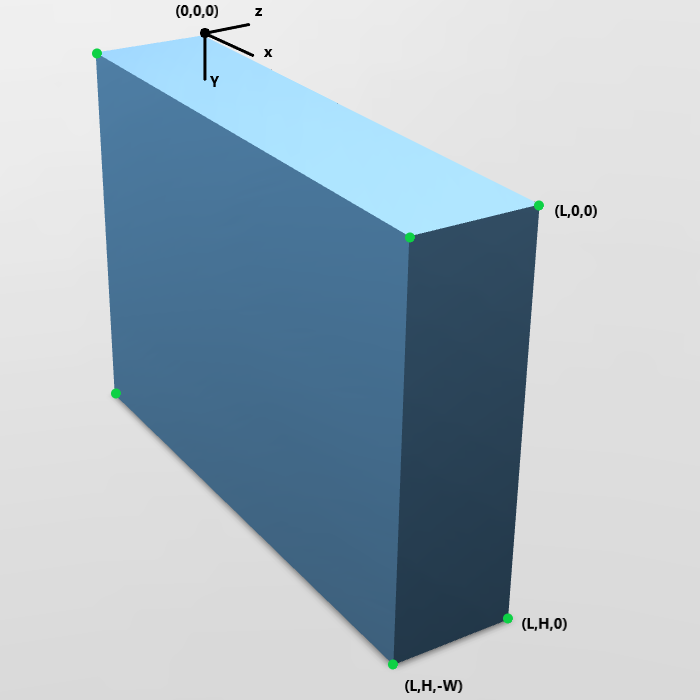
\includegraphics[width=0.75\textwidth]{BoxModel.png}
		\caption{Rigid object model.} \label{box}
	\end{minipage}\hfill
	\begin{minipage}{0.5\textwidth}
		\begin{center}
			\begin{tabular}[5pt]{| c| c|}
				\hline
				Parameter	& Value (cm) \\[0.5ex] 
				\hline 	
				$Length$& 45.6  \\ \hline 
				$Height$& 32.5  \\ \hline 
				$Width$& 10.1  \\ \hline 
			\end{tabular}
			\captionof{table}{Object Dimensions}\label{boxdim}
		\end{center}	
	\end{minipage}
\end{figure}

\noindent From this we de-vectorize the result of the SVD and obtain $\Pi_{est}$. Using this, all necessary components to describe the calibration and pose of the camera are extracted. From order reversing the standard QR decomposition we are able to obtain the scaling factor $\alpha$, the calibration matrix, and the rotation matrices corresponding to the given set of pixel coordinates. Using this information we can lastly find the translation vector associated with the system from the following equation,where $T^{'} = KT$, and is the rightmost column of $\Pi_{est}$: 

\begin{multicols}{2}
	\begin{equation}\label{Teq}
		T = \dfrac{K^{-1}T^{'}}{\alpha}
	\end{equation}\break
	\begin{equation}\label{xp}
		\chi^{pj} = \dfrac{\Pi_{est} X_0^j}{\lambda^j}
	\end{equation}\break
\end{multicols}


Using the information obtained from the algorithm, we next show the ability to project estimated pixel coordinates in to the image plane. These estimated pixel coordinates are described by Equation \ref{xp}.  From this we are able to qualitatively visualize the success of the algorithm in matching provided correspondence points (Figure \ref{pixcoords}). From the estimated pixel coordinates in noiseless reconstructions of the object we calculate the average root mean square error (RMSE) of the position between the true coordinates and their respective estimates in the object frame in order to establish the overall fidelity of the algorithm across multiple images taken with varying rotations, translations, and calibrations. In this case PRMSE is expressed by Equations \ref{dist} and \ref{PRMSE}, where $n_{im}$ is the number of images, and $n_{f} $ is the number of features used:
\begin{equation}\label{dist}
d_i = \sqrt{(x_o^{ij}-\hat{x}_o^{ij})+(y_o^{ij}-\hat{y}_o^{ij})+(z_o^{ij}-\hat{z}_o^{ij})}\quad \text{for} \quad j=1,2,...,n_{im}
\end{equation}
\begin{equation}\label{PRMSE}
	PRMSE =\dfrac{\sum_{j=1}^{n_{im}}\sqrt{\sum_{i=1}^{n_f}\sqrt{di/n_f}}}{n_{im}}
\end{equation}
\begin{figure}
	\centering % must do this or your figure won't be centered
	\includegraphics[width=0.55\textwidth]{pixcoords.eps}
	\caption{Estimated pixel coordinates} \label{pixcoords} 
\end{figure}
\noindent Across the four tested images (with no noise corruption) through 100 iterations of the algorithm, the average distance error was relatively small at $PRMSE = 0.2763 \quad$\ cm . 

\subsection{Corrupted Correspondence Points}
 Once the results of the algorithm are proven to work on its own data sets we observe the effect of the calibration and pose established by the algorithm on the pure data set (as opposed to the estimated) data to observe the distortions due to noise or error in correspondence. When applying normally distributed to each component of the correspondence points individually with a standard deviation of $\sigma = 100$ pixels we receive reconstruction results similar to those seen in \ref{noiseall}. From the calibration received, we test the ability to reconstruct the true (uncorrupted) data. This yields considerable disfigurement of the object. The reconstruction of the original box when corrupted by noise and the ground truth can seen in Figure \ref{noiseallrecon}.  To quantitatively capture the results of the noise reconstruction we compare the angles created between the correspondence points. Since the object is a box and the correspondence points lie along the edges, it is expected that all adjacent vectors are orthogonal to each other. 

\begin{figure}[h]
	\centering % must do this or your figure won't be centered
	\captionsetup{justification=centering}
	\begin{minipage}{0.5\textwidth}
		\centering
		\includegraphics[width=1\textwidth]{noise_all.eps}
		\caption{Estimated image coordinates \newline(unique coordinate component noise)} \label{noiseall}
	\end{minipage}\hfill
	\begin{minipage}{0.5\textwidth}
		\centering % must do this or your figure won't be centered
		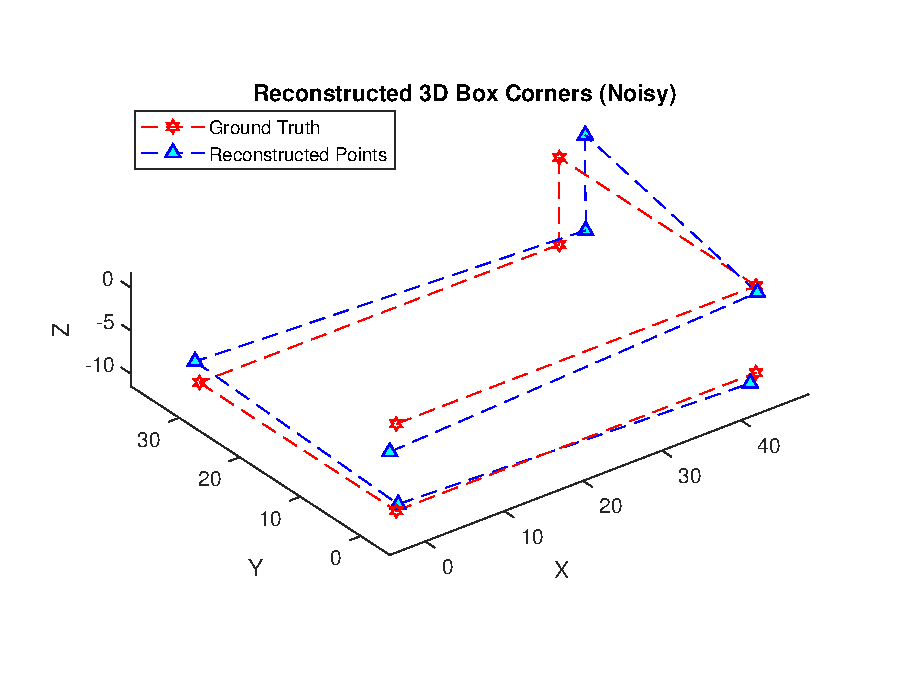
\includegraphics[width=1\textwidth]{noise_all_recon.eps}
		\caption{Reconstructed box relative to ground truth} \label{noiseallrecon}
	\end{minipage}
\end{figure}

\subsection{Improper Dimensions}



\section{Conclusions}



\appendix % this command sets sectioning command to the appendix format
% uncomment the next line to start on a fresh page
\newpage

\section{Code Listings}\label{code}

% input the file containing the code
%\lstinputlisting[caption={Top level implementation for Monocular Calibration and Pose Estimation},label={proj}]{MonoPose.m}
%\lstinputlisting[caption={QR Decomp Based Algorithm Implementation},label={alg}]{MonoPoseQR.m} 
%\lstinputlisting[caption={Rearranged QR Decomposition (Credit: Dr. John McInroy)},label={qrCom}]{qrCommute.m}
%\lstinputlisting[caption={Expectation Maximization, Version 2},label={EM2}]{EM2.m}
%\lstinputlisting[caption={Mixture Model PDF},label={prob}]{p.m}


%% The commands below automatically generate the References section
%% using the ``sample_bib'' file I've given you.

\newpage  % start a new page

\bibliographystyle{ieeetr}
\bibliography{a1_abbrv,Proj2}

\end{document} % always the last line of your document file
